% ### Uses XeLaTeX ### %
% ### Needs beamer-master ### %
\documentclass[aspectratio=169]{beamer} %. Aspect Ratio 16:9


%\patchcmd{\verb}{\dospecials}{\dospecials\atspecial}{}{}
%\def\atspecial{\begingroup\lccode`~=`@
%  \lowercase{\endgroup\let~}\MVAt
%  \catcode`@=\active}
  
  
\usetheme{AI2} % beamerthemeSprace.sty
% DATA FOR FOOTER
\date{2020}
\title{MLops}
\author{}
\institute{Advanced Institute for Artificial Intelligence (AI2)}
\usepackage{xcolor}

\usepackage{listings}


%eeeee
\usepackage{marvosym,etoolbox}

\lstset{literate={@}{\MVAt}1}

\patchcmd{\verb}{\dospecials}{\dospecials\atspecial}{}{}
\def\atspecial{\begingroup\lccode`~=`@
  \lowercase{\endgroup\let~}\MVAt
  \catcode`@=\active}
%eeeee

\begin{document}
% ####################################
% FIRST SLIDE 						:: \SliTit{This is the Title of the Talk}{A. B. Name}{Sprace}
% SUB-TITLE SLIDE 					:: \SliSubTit{<title>}{<explanation}
% SUB-SUB-TITLE SLIDE				:: \SliSubSubTit{<title>}{<explanation}
% SLIDE WITH TITLE 					:: \SliT{Title}{Content}
% SLIDE NO TITLE 						:: \Sli{Content} 
% SLIDE DOUBLE COLUMN WITH TITLE 	:: \SliDT{Title}{First Column}{Second Column}
% SLIDE DOUBLE COLUMN NO TITLE 		:: \SliD{First Column}{Second Column}
% SLIDE ADVANCED WITH TITLE 			:: \SliAdvT{Title}{Content}
% SLIDE ADVANCED NO TITLE 			:: \SliAdv{Content}
% SLIDE ADVANCED DOUBLE WITH TITLE 	:: \SliAdvDT{Title}{First Column}{Second Column}
% SLIDE ADVANCED DOUBLE NO TITLE 	:: \SliAdvD{First Column}{Second Column}
% SLIDE BLACK						:: \Black{ <Content> }
% SLIDE WHITE						:: \White{ <Content> }
% ITEMIZATION 						:: \begin{itemize}  \iOn{First} \iTw {Second} \iTh{Third} \end{itemize}
% COMMENT TEXT				 		:: \note{<comment>}
% SECTION 							:: \secx{Section} | \secxx{Sub-Section}
% BOLD SPRACE COLOR				:: \bfs{<text>}
% TABLE OF CONTENT					:: \tocitem{<title>}{<content>}
% LEFT ALIGN EQUATION				:: \begin{flalign*}  & <equation> &   \end{flalign*}
% CENTER ALIGN EQUATION	S			:: \begin{gather*} <equations>  \end{gather*}
% SLASH								:: \slashed{<>}
% BAR								:: \barr{<letter>} instead of \bar{<letter>}
% THEREFORE						:: use \portanto (larger and bold}
% 2 or 3 MATH SYMBOLS				:: \overset{<up>}{<down>} &  \underset{<below>}{\overset{<above>}{<middle>}}  
% INSERT TEXT IN FORMULA			:: \ins{<text>}
% EXERCISE							:: \exe{<exercise #>}{<exercise text>}
% SUGGESTED READING BOX			:: \sug{<references>}
% CITATION							:: \cittex{<citation>}
% CITATION DOUBLE COLUMN 			:: \cittexD{<citation>}
% TEXT POSITION						:: \texpos{<Xcm>}{<Ycm>}{<text>} origin = center of slide : x right | y down
% REFERENCE AT BOTTOM  S/D SLIDE		:: \refbotS{<reference>} \refbotD{<reference>}
% HIDDEN SLIDE						:: \hid
% COLOR BOX 						:: \blu{blue} + \red{rec} + \yel{yellow} + \gre{green} + \bege{beige}
% FRAME 							:: \fra{sprace} \frab{blue} \frar{red} + \fray{yellow} + \frag{green}		
% FIGURE 							:: \img{X}{Y}{<scale>}{Figure.png} 
% FIGURE							:: \includegraphics[scale=<scale>]{Figures/.png}
% FIGURE DOUBLE SLIDE NO TITLE		::  \img{-4}{0.5}{<scale>}{Figure.png} % Image 1st half
%									::  \img{4}{0.5}{<scale>}{Figure.png} % Image 2nd half
% FIGURE DOUBLE SLIDE WITH TITLE		::  \img{-4}{0}{<scale>}{Figure.png} % Image 1st half
%									::  \img{4}{0}{<scale>}{Figure.png} % Image 2nd half
% INCLUDING SWF (Flash)				:: \usepackage{media9} and \includemedia >> USE ACROBAT <<
%%%%%%%%%%%%%%%%%%%%%%%%%%%%%%%%%%%%%%%%%%%%%%%%%%
% ###############################################################################
% FIRST SLIDE
\SliTit{MLops}{Advanced Institute for Artificial Intelligence -- AI2}{https://advancedinstitute.ai}
%%%%%%%%%%%%%%%%%%%%%%%%%%%%%%%%%%%%%%%%%%%%%%%%%%
% ###############################################################################
% SLIDE SUB-TITLE
%\SliSubTit{Sub-Title}{Description}{}
%%%%%%%%%%%%%%%%%%%%%%%%%%%%%%%%%%%%%%%%%%%%%%%%%%
% ###############################################################################
%\SliSubSubTit{Sub-Sub-Title}{Description}
 %%%%%%%%%%%%%%%%%%%%%%%%%%%%%%%%%%%%%%%%%%%%%%%%%%
% ###############################################################################
% SLIDE WITH TITLE

\SliT{Agenda}{
    Agenda
    
    \begin{itemize}
       \iOn{Integração e Entrega Contínua}
       \iOn{Fluxo de Trabalho de Aplicações de Aprendizagem de Máquina}
       \iOn{Introdução ao Modelo de Microserviços}
       \iOn{Automação de Fluxo de Dados (DATAOps)}
       \iOn{Automação de Montagem e Avaliação de Aplcações de Aprendizagem de Máquina (MLOps)}
   \end{itemize}
}


\SliT{Desenvolvimento Contínuo}{


\begin{itemize}
\iOn{Integracao continua (CI): desenvolvedor continuamente integra seu código (normalmente uma ramificação do código principal) com o código principal}
\iTw{Controle de versão}
\iTw{Build automatizado}
\iTw{Check in frequente}
\iTw{Suíte de testes abrangente}
\iOn{Entrega continua (CD): processo automatizado que permite colocar uma nova versão do código principal em produção e desfazer o processo caso ocorra problemas, de forma simples}
\iTw{Colocar em producao automaticamente}
\iTw{Automacao de uso de conteineres}
\iTw{Integracao continua é um pré-requisito}
\iTw{Normalmente um processo semi-automático}

\iOn{Montagem (Deploy) Contínua: todo código que entra na master automaticamente é colocado em produção}

\end{itemize}

}

\SliT{Desenvolvimento Contínuo} {
\begin{center}
    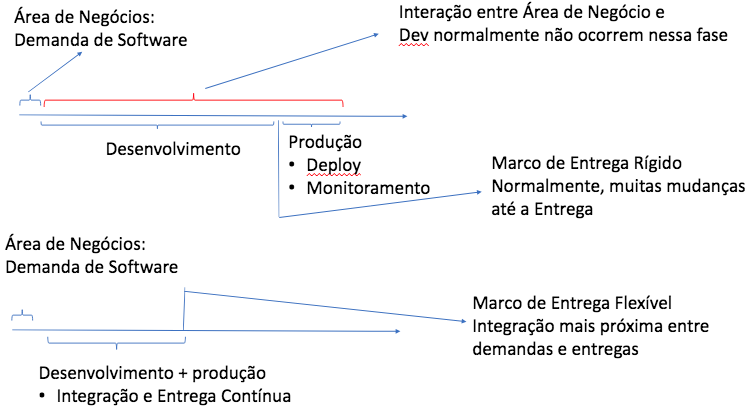
\includegraphics[scale=0.50]{figs/1.png}
\end{center}
}

\SliT{Desenvolvimento Contínuo}{

Integracao e Entrega Contínua representam uma flexibilizacao de entrega de software em marcos pré-definidos

\begin{itemize}
\iOn{Maior sinergia entre demandantes de software e processo de desenvolvimento de software}

\iOn{Desenvolvimento de software pode ser feito de modo mais granular}

\iOn{Cada nova funcionalidade pode ser desenvolvida e implantanda sem impactar o sistema como um todo}

\iOn{Permite melhorar o atendimento de expectativas da área de negócios, que pode ter novas funcionalidades disponíveis em curtos espaços de tempo}

\iOn{Processo auto controlado, que permite organizar o trabalho, mantendo a liberdade de cada colaborar de utilizar usas próprias ferramentas }

\end{itemize}

}

\SliT{Desenvolvimento Contínuo}{

Como alcançar tais níveis de automação?

\begin{itemize}

\iOn{Profissional TI dedicado a colocar sistemas diversos em produção}
\iTw{Pouco ou nenhum conhecimento da estrutura de tais sistemas}
\iTw{Desenvolvedores do sistema possuem pouco ou nenhum conhecimento quanto a montagem de tais sistemas}

\iOn{Barreira entre desenvolvimento e produção} \iTw{Dependencias normalmente desconhecidas}
\iTw{Complexidade das etapas desconhecidas}

\iOn{Integração/Entrega contínua é uma forma de quebra tal barreira}
\iTw{Colocar um sistema em producao, ou uma parte dele, é um processo conhecido pelo desenvolvedor e TI}
\iTw{Processo claro, planejável e conhecido usando especificações comuns}
\end{itemize}  

}

\SliT{Desenvolvimento Contínuo}{

\begin{itemize}
\iOn{OPs Contração que mostra unificação de áreas com a parte operacional de colocar em produção}

\iOn{DEVOPs: prática de software que unifica o desenvolvimento de software (Dev) e a operação de software (Ops)}

\iOn{Tecnologias diversas como Git, Jenkins, tecnologias de teste automatizados, usando por equipes compostas por desenvolvedores e TI}
\iOn{As mesmas práticas de DEVOps tem sido também se popularizado para desenvolvimento de sistemas de aprendizagem de máquinas:}
\iTw{CD4ML}
\iTw{DATAOPs}
\iTw{MLOPs}
\end{itemize}

}

\SliT{Desenvolvimento Contínuo}{

Sistemas de aprendizagem de máquina (Machine Learning), são tipos de sistemas que seguem uma estrutura clara

\begin{itemize}
\iOn{Organizacao dos dados de entrada}
\iOn{Desenvolvimento de um modelo}
\iOn{Avaliacao do modelo}
\iOn{Colocar modelo em produção}
\iOn{Receber requisições para predição}

\end{itemize}  
}


\SliT{Desenvolvimento Contínuo} {
\begin{center}
    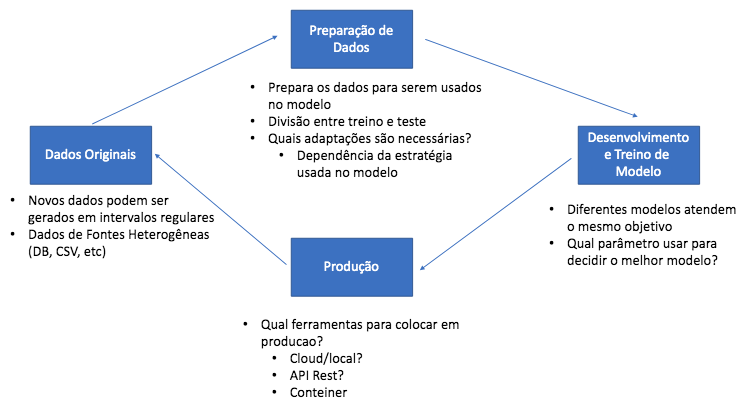
\includegraphics[scale=0.45]{figs/2.png}
\end{center}
}



\SliT{Desenvolvimento Contínuo}{

Melhorias contínuas podem ser feitas em aplicações de Apredizagem de Máquina considerando diferentes aspectos:
\begin{itemize}
\iOn{Organizar os dados usados para treino que são gerados diariamente}
\iOn{Adaptar modelos para utilização de dados complementares}
\iOn{Comparação entre modelos implementados de acordo com dferentes abordagens}
\iOn{Implementar modelos que abordam o problema de outras maneiras}
\iOn{Adaptações quanto a forma de integração do modelo com outras aplicações}
\iOn{Adequações para melhorar o desempenho do treino e predição}
\end{itemize}  
}



\SliT{Desenvolvimento Contínuo}{

Ferramentas para desenvolvimento de microserviços:

\begin{itemize}
\iOn{Flask biblioteca para Microserviço}
\iOn{Json protocolo para troca de dados}
\end{itemize}

}

\SliT{Desenvolvimento Contínuo}{


\begin{itemize}
\iOn{O framework Flask permite criar servidores web seguindo a especificaçáo WSGI (Web Server Gateway Interface), que é um padrão para o desenvolvimento de aplicações web em Python}

\iOn{A idéia desse padrão é permitir a portabilidade de uma aplicação web em python entre diferentes servidores web atuando como um middleware}

\iOn{Flask provê recursos para}

\iTw{Iniciar um servidor web}
\iTw{Capturar as chamadas para diferentes funcionalidades de acordo com as URLs passadas}
\iTw{processas as requisições em um script python}
\end{itemize}

}

\begin{SliTC}{Código em Shell}
Instalando flask

\begin{lstlisting}[language=bash]
pip install flask
\end{lstlisting}
\end{SliTC}

\begin{SliTC}{Desenvolvimento Contínuo}

Uma aplicação mínima em Flask precisa importar a class Flask, criar uma instância da classe flask e atender ao menos uma requisição web

O Routing define um formato de URL que deve ser capturado e direciona a chamada para uma função escrita em python

Para isso vamos salvar o código a seguir em um arquivo chamado flaskapp.py

\begin{lstlisting}[language=Python]
from flask import Flask
app = Flask(__name__)

app.route('/')
def hello_world():
    return 'Hello, World!'
    
\end{lstlisting}

\end{SliTC}

\begin{SliTC}{Desenvolvimento Contínuo}

Para colocarmos o microserviço em produção é necessário executar dois passos:

Criar a variável de ambiente FLASK\_APP e atribuir como valor o nome do arquivo criado (flaskapp)

\begin{lstlisting}[language=bash]
export FLASK_APP=flaskapp
\end{lstlisting}

Executar o ambiente flask:

\begin{lstlisting}[language=bash]
flask run
\end{lstlisting}

\end{SliTC}


\begin{SliTC}{Desenvolvimento Contínuo}
 
 Isso indica que o servidor está no ar no local host e respondendo na porta TCP 5000. Por ser um servidor web, podemos realizar chamadas a ele por meio do navegador

O Código a seguir mostra como implementar uma requisição passando parâmetros

\begin{lstlisting}[language=Python]
from flask import Flask
app = Flask(__name__)

app.route('/user/<username>')
def profile(username):
    return username
\end{lstlisting}
\end{SliTC}


\SliT{Desenvolvimento Contínuo} {

\begin{itemize}

\iOn{O parâmetro @app.route() define qual URL será tratada pelo servidor.}

\iOn{Ao capturar essa URL o servidor direcionará a chamada a função declarada na próxima linhas após o @app.route que é a função hello\_world()}

\iOn{Essa função tem como objetivo retornar uma string com o valor "Hello, World!"}

\iOn{Esse retorno é direcionado como resposta ao cliente (Nesse caso um navegador) que realizou a chamada ao servidor web, portanto vai mostrar na tela do navegador a mensagem : "Hello, World!"}

\end{itemize}

}



\begin{SliTC}{Desenvolvimento Contínuo}

\begin{itemize}

\iOn{Podemos também realizar chamadas a um microserviço por meio de uma aplicação python.

\iOn{Para realizar uma requisição web vamos utilizar a biblioteca urllib.request (https://docs.python.org/3/library/urllib.request.html)

\iOn{Essa biblioteca permite realizar requisições a servidores web em python

\iOn{insira o código a seguir em um script chamado cliente.py
\end{itemize}

\begin{lstlisting}[language=Python]

import urllib.request
contents = urllib.request.urlopen("http://localhost:4000/user/user2").read()

print(type(contents))
print(contents)
\end{lstlisting}
\end{SliTC}



\SliT{Desenvolvimento Contínuo} {

\begin{itemize}

\iOn{REST (Representational State Transfer): Um aplicativo Web RESTful expõe informações sobre si na forma de informações sobre seus recursos. Ele também permite que o cliente execute ações nesses recursos, como criar novos recursos (por exemplo, criar um novo usuário) ou alterar os recursos existentes (por exemplo, editar uma postagem).}

\iOn{Um aplicativo REST é utilizado por meio de requisições HTTP e provê respostas do tipo HTML, XML ou Json}
\iOn{É como requisitar uma URL no navegador e receber uma página HTML como resposta. A diferença é que a solicitação via REST é feita a uma aplicação e não para um arquivo estático}
\iOn{Json (JavaScript Object Notation): é um formato bastante flexível para determinar a forma como as aplicações se comunicam.}

\end{itemize}
}

\begin{SliTC}{Desenvolvimento Contínuo}

O código abaixo modifica a função de buscar a idade do cliente para retornar um objeto json
    \begin{lstlisting}[language=Python]

from flask import jsonify

app.route('/busca/<username>')
def searchuser(username):
	idade=0
	with open('clientes.txt') as f:
		for line in f: 
			l=line.split(';')
			if (l[0] == username):
				idade=l[1]	
	return jsonify(cliente= username, idade= idade)
	    \end{lstlisting}
\end{SliTC}

\begin{SliTC}{Desenvolvimento Contínuo}

O Cliente pode realizar o parser das informações enviadas usando a lib json conforme o código abaixo:

\begin{lstlisting}[language=Python]
import json

def buscarCliente():
	nome = input("Digite o nome do cliente que deseja buscar: ")
	
	contents = urllib.request.urlopen("http://127.0.0.1:5000/busca/"+nome).read()

	print(contents)
	cliente_idade = json.loads(contents)
	print(cliente_idade['cliente'])
	print(cliente_idade['idade'])
	
\end{lstlisting}

\end{SliTC}

\SliT{Desenvolvimento Contínuo} {
\begin{center}
    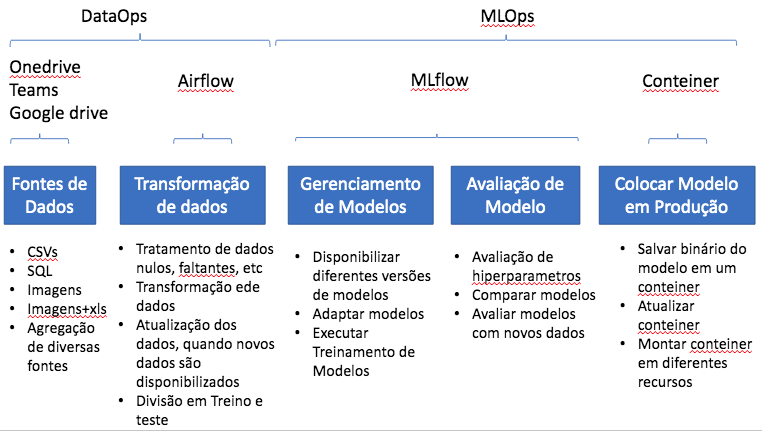
\includegraphics[scale=0.45]{figs/3.png}
\end{center}
}
\SliT{Desenvolvimento Contínuo} {
ETL (Extract, Transform and Load) Extração Transformação e Carga é um processo para integração de dados de fontes distintas. A idéia é construir uma base de dados centralizada por meio de três passos:

\begin{itemize}

\iOn{Extração dos dados de diferentes fontes}
\iOn{Transformação dos dados para um formato que permita a análise conjunta dos dados}
\iOn{Carga dos dados em um repositório com todas as informações em um único local}
\end{itemize}

}

\SliT{Desenvolvimento Contínuo} {
É comum utilizar ETL para diversos processos:
\begin{itemize}

\iOn{integrar dados de múltiplos sistemas, e obter uma visão unificada de um processo que passa por todos esses sistemas}
\iOn{integrar com dados de fontes externas}
\iOn{preparar os dados para uma análise específica}
\end{itemize}

}

\SliT{Desenvolvimento Contínuo} {

\begin{itemize}
\iOn{Algoritmos de Aprendizagem de Máquina normalmente são treinados em um conjunto de dados preparado adequadamente}

\iOn{É comum que a obtenção, preparação  e gerenciamento dos dados seja feito por um profissional especializado nessa atividades (chamado engenheiro de dados), por ser um processo complexo e independente do desenvolvimento do modelo de aprendizagem de máquina}

\iOn{Ferramentas que automatizam essa etapa são essenciais para permitir uma melhor integração entre o trabalho do engenheiro de dados e o cientista de dados}
\iTw{Essa integração é chamada de DataOps}

\end{itemize}

}

\SliT{Desenvolvimento Contínuo} {


DataOps 
\begin{itemize}
\iOn{uma metodologia automatizada com base no processo de desenvolvimento de algoritmos de aprendizagem de máquina}

\iOn{Melhora a qualidade dos dados e reduz o tempo de análise de dados}
\iOn{Basedo na metodologia ágil e no conceito de entrega contínua}
\iOn{Diversas ferramentas permitem implementar esse processo}
\end{itemize}
}

\SliT{Desenvolvimento Contínuo} {
Apache Airflow é uma ferramenta aberta de DataOps

\begin{itemize}
\iOn{Permitir especificar workflows capazes de extrair informação de fontes de dados e aplicar transformações diversas para gerar um dataset adequado ao cientista de dados.}

\iOn{As tarefas do workflow podem ser implementadas em diversas linguagens como o Python por exemplo}

\iOn{Os workflows podem ser agendados para rodar em intervalos regulares}
\iTw{Dessa forma, é possível manter um dataset relativo a um processo que ocorre todo dia sempre atualizado}

\iOn{A colaboração entre o engenheiro de dados e o cientista de dados pode entao ser completamente gerenciada pela ferramenta de DataOps Apache Airflow}
}

\end{itemize}
}


\begin{SliTC}{Desenvolvimento Contínuo}

A seguir a estrutura de um código que implementa um DAG em Airflow (Tarefas implementadas em Python)

\begin{lstlisting}[language=Python]
from airflow import DAG
from airflow.operators.python_operator import PythonOperator

def prep_cliente():
    
    print('task1')
    
def prep_cliente_perfil():
    
    print('task2')   
    
\end{lstlisting}

\end{SliTC}


\begin{SliTC}{Desenvolvimento Contínuo}
Criação do DAG

\begin{lstlisting}[language=Python]
    
default_args = {
    'owner': 'airflow',
    'depends_on_past': False,
    'email': ['airflow at example.com'],
    'email_on_failure': False,
    'email_on_retry': False,
    'retries': 1
}

dag = DAG(
    'prep_sicoob',
    default_args=default_args,
    description='DAG de preparacao de dados para Sicoob'
)

\end{lstlisting}

\end{SliTC}

\begin{SliTC}{Desenvolvimento Contínuo}
Referencia as tarefas

\begin{lstlisting}[language=Python]

prep_cliente = PythonOperator(task_id='prep_cliente',
                                 python_callable=prep_cliente, dag=dag,)
prep_cliente_perfil = PythonOperator(task_id='prep_cliente_perfil',
                                 python_callable=prep_cliente_perfil, dag=dag,)
\end{lstlisting}
Sequência da execução das tarefas
\begin{lstlisting}[language=Python]
prep_cliente >>  prep_cliente_perfil
\end{lstlisting}

\end{SliTC}


\SliT{Desenvolvimento Contínuo} {


\begin{itemize}
\iOn{Ao terminar o desenvolvimento do DAG é necessário armazena-lo e executa-lo no terminal}
\iOn{O DAG estará disponível para ser executado a partir da interface gráfico do Airflow}

\end{itemize}

}

\SliT{Desenvolvimento Contínuo} {
\begin{itemize}
\iOn{O processo de desenvolvimento de modelo de aprendizagem de máquina de modo geral se baseia em um objetivo (normalmente definido em termos de uma predição) e um conjunto de dados}

\iOn{Para um mesmo objetivo de conjunto de dados diversos modelos podem ser criados, a diferença entre eles está na qualidade alcançada}

\iOn{A qualidade normalmente é medida em termos de métricas estatísticas}

\end{itemize}

}


\SliT{Desenvolvimento Contínuo} {

\begin{itemize}
\iOn{Nesse cenário a integração e entrega contínua nesse processo é fundamental, pois a comunicação entre Cientistas de Dados e a equipe de operações ou produção é fundamentamente colaborativa}

\iOn{Tal colaboração precisa ser automatizada para colocar sistemas de aprendizagem de máquina em produção mais rápido e minimizar os riscos}

\iOn{MLOps (uma combinação de Machine Learning e “operações de tecnologia da informação”) é uma nova disciplina / foco / prática para colaboração e comunicação entre Cientistas de Dados e profissionais de tecnologia da informação (TI)}
\end{itemize}
}

\SliT{Desenvolvimento Contínuo} {
\begin{itemize}
\iOn{Ferramentas para colocar sistemas de aprendizagem de máquina em produção são normalmente chamados de serving systems}

\iOn{A idéia do serving systems é criar uma interface de microserviços que receba uma requisião para uma predição e retorne a predição}

\iOn{A utilização de microserviços é essencial para permitir maior flexibilidade quanto a desempenho, segurança, montagem e integração do módulo de predição em diversas aplicações}
\end{itemize}
}

\SliT{Desenvolvimento Contínuo} {

Um exemplo de Serving System em Tensorflow é o tensorflow\_model\_server

\begin{itemize}

\iOn{Modelo em Keras é salvo para o disco}

\iOn{Modelo é carregado por um sistema que recebe requisições REST para fazer predições}

\end{itemize}

Outras ferramentas para automatizar o processo de desenvolvimento de aplicações de aprendizagem de máquina também são disponibilizadas pelo tensorflow

}

\SliT{Desenvolvimento Contínuo} {

O MLFlow é um exemplo de ferramenta que automatiza e facilita o controle do desenvolvimento de aplicações de aprendizagem de máquina

\begin{itemize}
\iOn{O MLflow apresenta as seguintes funcionalidades:}
\iTw{Permite armazenar métricas de qualidade de diversos modelos relacionados a um mesmo experimento}
\iTw{Permite gerar o executável do modelo a partir de diversos frameworks}

\end{itemize}
}




\end{document}
